\chapter{Matrices multiplication}

The code of the non-optimized version of this program can be found in the appendix \ref{matmul} and that of the optimized version in the appendix \ref{matmulot}. 
The optimization done in the version is simply an inversion of the two inner loops used to perform the matrices multiplication. It optimizes the use of the cache and this is enough to speed the program up considerably.

The picture \ref{matmul} presents the results.

\begin{figure}[!h]
  \begin{center}
         \resizebox{160mm}{!}{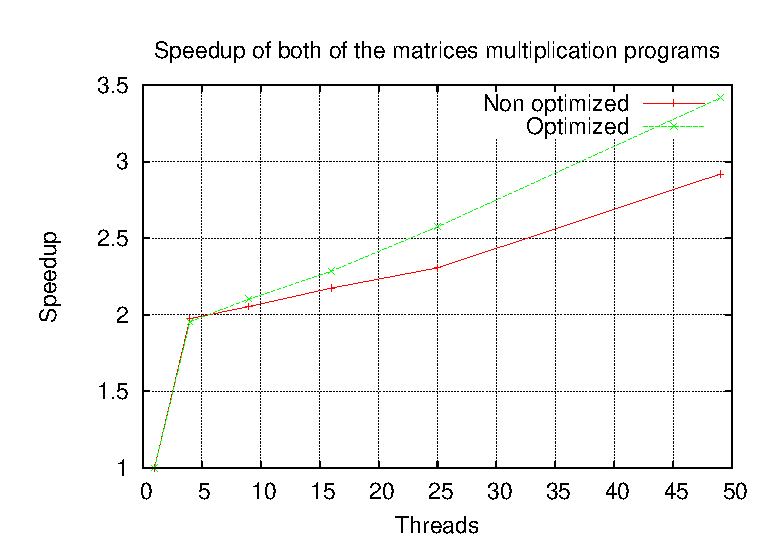
\includegraphics{pic/graph_matmul.eps}}
  \end{center}
  \caption{Speedup of both of the matrices multiplication programs}
  \label{matmul}
\end{figure}

As we can see on the diagram, performances are better with the cache optimisation of the second version. This shows the importance of knowing how data is stored in the computer and how to optimize the access to it.

